\section{Registrazione}
All'avvio di \textit{Gaiago} viene presentata la schermata per effettuare il login. Premendo la scritta "registrati" di colore verde si viene portati alla fase di registrazione.
\begin{figure}[H] 
	\centering 
	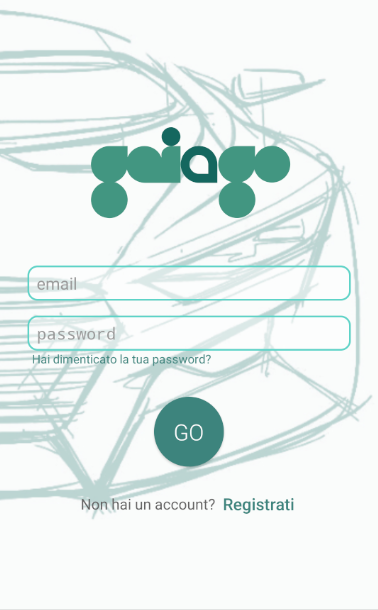
\includegraphics[width=0.5\textwidth]{res/images/login.png}\\
	\caption{Fase di login}
	\label{Login}
\end{figure}
 \pagebreak
Come si può vedere dalla figura sottostante per effettuare la registrazione è necessario compilare tutti i campi previsti:
\begin{itemize}
	\item \textbf{email}
	\item \textbf{password}
	\item \textbf{conferma password}
\end{itemize} 

I campi vanno compilati singolarmente cliccando sul corrispettivo input di testo con relativo placeholder in grigio chiaro che indica cosa inserire. Una volta compilati tutti i campi si preme il bottone "AVANTI". Se sono stati rispettati tutti i vincoli la registrazione prosegue altrimenti sarà necessario rivedere i dati inseriti e correggerli di conseguenza. 
 \begin{figure}[H] 
 	\centering 
 	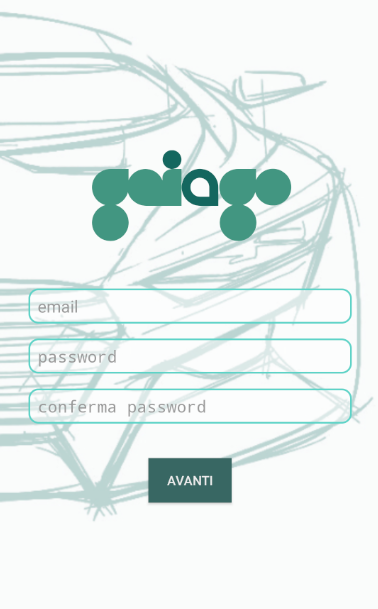
\includegraphics[width=0.5\textwidth]{res/images/registrazione.png}\\
 	\caption{Fase di login}
 	\label{Login}
 \end{figure}

\pagebreak

Per completare la registrazione dell'account è richiesto di inserire anche il nome e cognome dell'utente come si vede dalla figure seguente.
 \begin{figure}[H] 
	\centering 
	
\includegraphics[width=0.5\textwidth]{res/images/registrazione2.png}\\
	\caption{Fase di login}
	\label{Login}
\end{figure}

Una volta inseriti il nome e cognome, i quali non hanno richieste particolari di formato, per completare la registrazione e creare l'account si preme il bottone "CREA ACCOUNT" di colore verde.

\subsection{Guida introduttiva}
Al termine della registrazione prima di utilizzare l'applicazione viene mostrata all'utente una guida introduttiva, la quale funge da tutorial\glosp per aiutare ad apprendere le meccaniche essenziali di \textit{Gaiago}.

